\documentclass{article}


\usepackage{arxiv}

%\usepackage[utf8]{inputenc} % allow utf-8 input
\usepackage[T1]{fontenc}    % use 8-bit T1 fonts
\usepackage{hyperref}       % hyperlinks
\usepackage{url}            % simple URL typesetting
\usepackage{booktabs}       % professional-quality tables
\usepackage{amsfonts}       % blackboard math symbols
\usepackage{nicefrac}       % compact symbols for 1/2, etc.
\usepackage{microtype}      % microtypography
\usepackage{lipsum}
\usepackage{graphicx}
\usepackage{subfig}
%\usepackage{subcaption} 
%\graphicspath{ {./images} }
\usepackage[rightcaption]{sidecap}
\usepackage{wrapfig}
\usepackage{amsmath}
\usepackage{fancyvrb}
\usepackage{braket}
\usepackage{bbold}

\usepackage{todonotes}


\usepackage{listings}
\usepackage{color}

\definecolor{dkgreen}{rgb}{0,0.6,0}
\definecolor{gray}{rgb}{0.5,0.5,0.5}
\definecolor{mauve}{rgb}{0.58,0,0.82}

\lstset{frame=tb,
  language=C++,
  aboveskip=3mm,
  belowskip=3mm,
  showstringspaces=false,
  columns=flexible,
  basicstyle={\small\ttfamily},
  numbers=none,
  numberstyle=\tiny\color{gray},
  keywordstyle=\color{blue},
  commentstyle=\color{dkgreen},
  stringstyle=\color{mauve},
  breaklines=true,
  breakatwhitespace=true,
  tabsize=3
}

\title{Restricted Boltzmann machine representation for the groundstate and excited states of Kitaev Honeycomb model}


\author{
    Mohammadreza Noormandipour\thanks{\texttt{mrn31@cam.ac.uk}}\hspace{1mm}$^{,a}$ , Youran Sun\thanks{\texttt{syouran0508@gmail.com}}\hspace{1mm}$^{,b}$ , Babak Haghighat\thanks{\texttt{babakhaghighat@tsinghua.edu.cn}}\hspace{1mm}$^{,b}$ \\
	$^{a}$ \textit{DAMTP}, University of Cambridge, Wilberforce Road, Cambridge CB3 0WA, UK \\
	$^{b}$ \textit{Yau Mathematical Sciences Center}, Tsinghua University, Beijing, 100084, China\\
      %% David S.~Hippocampus\thanks{Use footnote for providing further
  %%  information about author (webpage, alternative
  %%    address)---\emph{not} for acknowledging funding agencies.} \\
  %% Department of Computer Science\\
  %% Cranberry-Lemon University\\
  %% Pittsburgh, PA 15213 \\
  %% \texttt{hippo@cs.cranberry-lemon.edu} \\
  %% examples of more authors
  %% \And
 %% Elias D.~Striatum \\
  %% Department of Electrical Engineering\\
  %% Mount-Sheikh University\\
  %% Santa Narimana, Levand \\
  %% \texttt{stariate@ee.mount-sheikh.edu} \\
  %% \AND
  %% Coauthor \\
  %% Affiliation \\
  %% Address \\
  %% \texttt{email} \\
  %% \And
  %% Coauthor \\
  %% Affiliation \\
  %% Address \\
  %% \texttt{email} \\
  %% \And
  %% Coauthor \\
  %% Affiliation \\
  %% Address \\
  %% \texttt{email} \\
}

\begin{document}
\maketitle

\begin{abstract}
%\lipsum[1]
In this work, the capability of restricted Boltzmann machines (RBMs) to find solutions for the Kitaev honeycomb model is investigated. The measured groundstate (GS) energy of the system is compared and shown to reside within less than $5\%$ error of the analytically derived value of the energy. Furthermore, the possibility of realizing anyons in the RBM is discussed and an algorithm is given to build these anyonic excitations and braid them as a proof of concept for performing quantum gates and doing quantum computation. Moreover, the phase transition of the system is also studied by changing the corresponding hyperparameters of the system in the RBM solution.
\end{abstract}


% keywords can be removed
\keywords{Restricted Boltzmann Machine (RBM) \and Honeycomb Lattice Model \and Topological Phases of Matter \and Anyons \and Quantum Computing}


\section{Introduction}
%\lipsum[2]
%\lipsum[3]
Honeycomb model is a 2-dimensional lattice spin system (see Fig.\hspace{0.2mm}\ref{fig:fig0}) which was first introduced by Kitaev in 2006 \cite{Kitaev_2006} and is famous because of the topological quantum order due to a degenerate gapped groundstate which is persistent to local and finite-sized perturbations. The system also supports both abelian and non-abelian topological phases as demonstrated in the original proposal \cite{Kitaev_2006}. There is a wide range of applications for this model, from fault-tolerant quantum computation \cite{Kitaev_2003} to analytical study of strongly correlated systems \cite{Jackeli_2009} and quantum spin liquids \cite{Tikhonov_2011}. The honeycomb lattice is not a Bravias lattice in its original structure, but it can be considered as a triangular Bravias lattice with a two-spin basis. The direct Bravias lattice and the primitive cells are illustrated in Fig.\hspace{0.2mm}\ref{fig:fig0}a with the dashed lines. Each primitive cell has a pair of odd and even indexed spins. Just for the sake of simplicity we will denote each cell with the even indexed (empty circles) spins of the system. The primitive vectors of the lattice, $\textbf{a}_1$ and $\textbf{a}_2$ are also shown in Fig.\hspace{0.2mm}\ref{fig:fig0}a (see also Equ.\hspace{0.2mm}\ref{eq:0}). The entire lattice can be tiled and covered with primitive cells using translations composed of different linear combinations of primitive vectors. 

\begin{equation}\label{eq:0}
    \textbf{a}_1 = \sqrt{3} a \textbf{e}_x \hspace{1cm} \& \hspace{1cm}
    \textbf{a}_2 = \frac{\sqrt{3}}{2} a (\textbf{e}_x, \sqrt{3}\textbf{e}_y)
\end{equation}

Where $a$ is the lattice constant. The reciprocal lattice for the triangle lattice can be obtained by solving Equ.\hspace{0.2mm}\ref{eq:01} for basis vectors of the reciprocal lattice, $\textbf{b}_1$ and $\textbf{b}_2$.

\begin{equation}\label{eq:01}
    \textbf{a}_i.\textbf{b}_j = 2\pi\delta_{ij}
\end{equation}

The solution is as below:

\begin{equation}\label{eq:02}
    \textbf{b}_1 = \frac{2\pi}{\sqrt{3}a} (\textbf{e}_x-\frac{1}{\sqrt{3}}\textbf{e}_y) \hspace{1cm} \& \hspace{1cm}
    \textbf{b}_2 = \frac{4\pi}{3a} \textbf{e}_y
\end{equation}

The reciprocal lattice is depicted in Fig.\hspace{0.2mm}\ref{fig:fig0}b. 

The Hamiltonian of the Kitaev model is a nearest-neighbor interaction of Pauli matrices on a honeycomb lattice as written in Equ.\hspace{0.2mm}\ref{eq:1}, where $r \& r^{'}$ are indices for the nearest neighbour spins. The physics of the system is symmetric under permutation of coupling strengths $J_{\alpha}$ with $\alpha = x, y, z$ and due to an-isotropic interaction the model is a fraustrated spin system, because a spin cannot satisfy conflicting
 demands of orientation from its three neighboring sites \cite{Kitaev_2006}.

\begin{equation}\label{eq:1}
    H = - \sum_{\alpha} J_{\alpha} \sum_{\alpha-bonds} \sigma^{\alpha}_{r}\sigma^{\alpha}_{r^{'}}
\end{equation}

\begin{figure}[h!]
%     \begin{subfigure}
     \centering
%     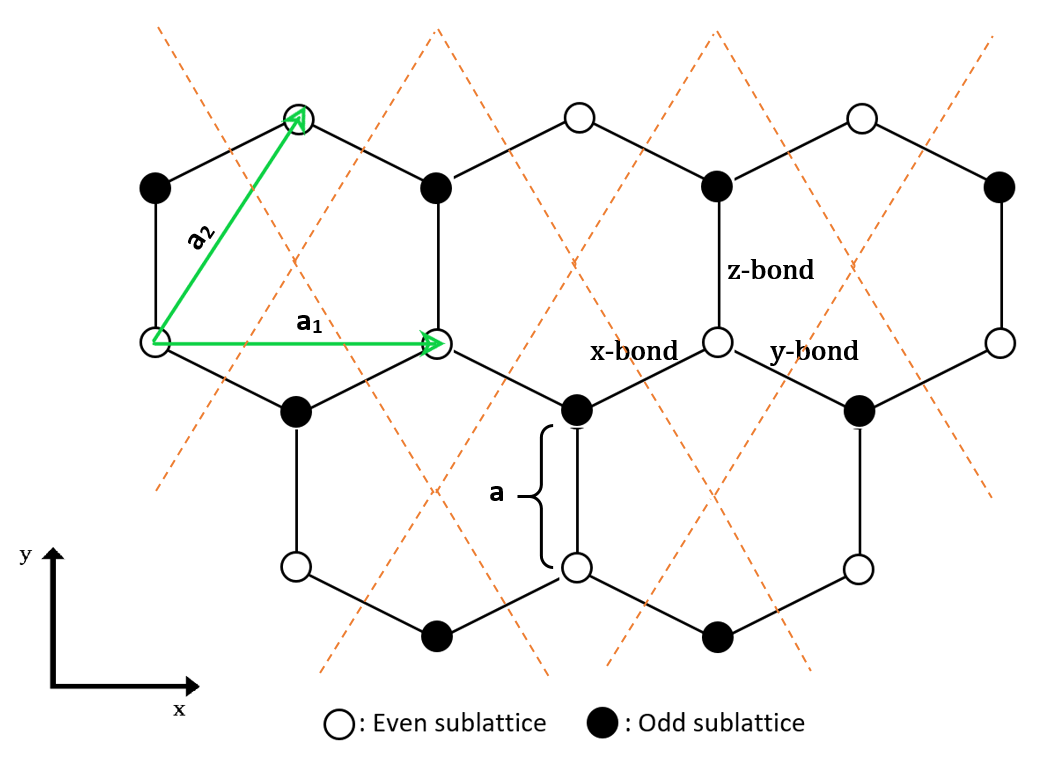
\includegraphics[width=0.8\textwidth]{./images/Final_A_2}
%     \caption{1a}
%     \label{fig:fig0a}
%     \end{subfigure}%
% 	\begin{subfigure}
%     \centering
%     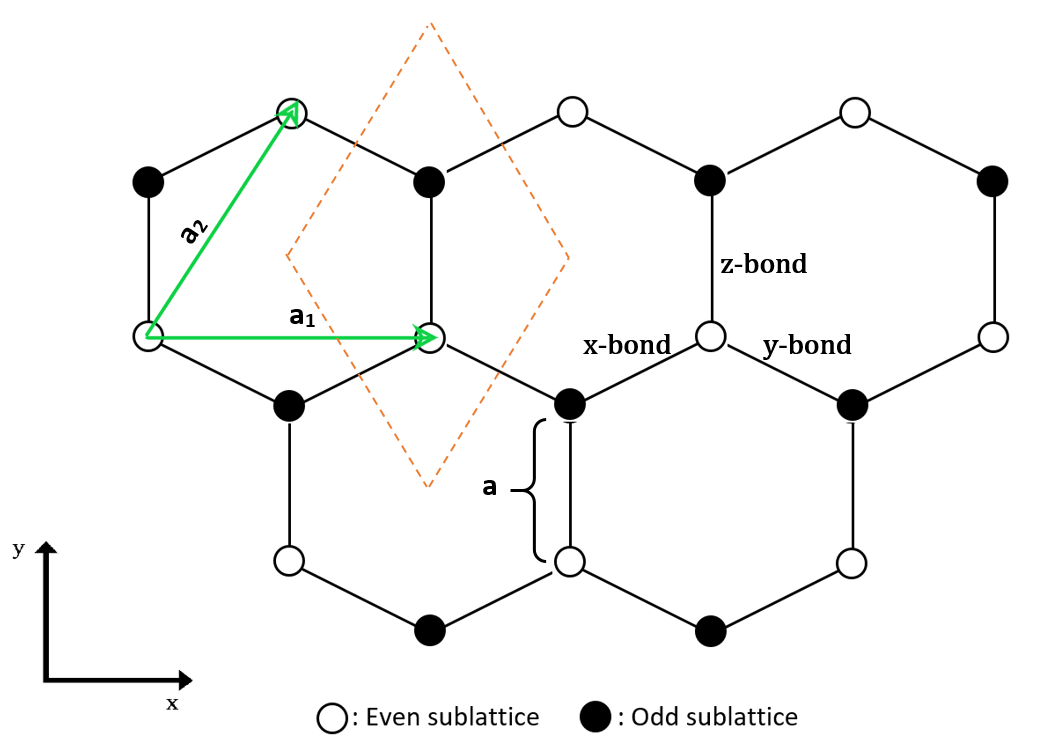
\includegraphics[width=0.8\textwidth]{./images/Final_A}
%     \caption{1b}
%     \label{fig:fig0b}
%     \end{subfigure}%
    \subfloat[]{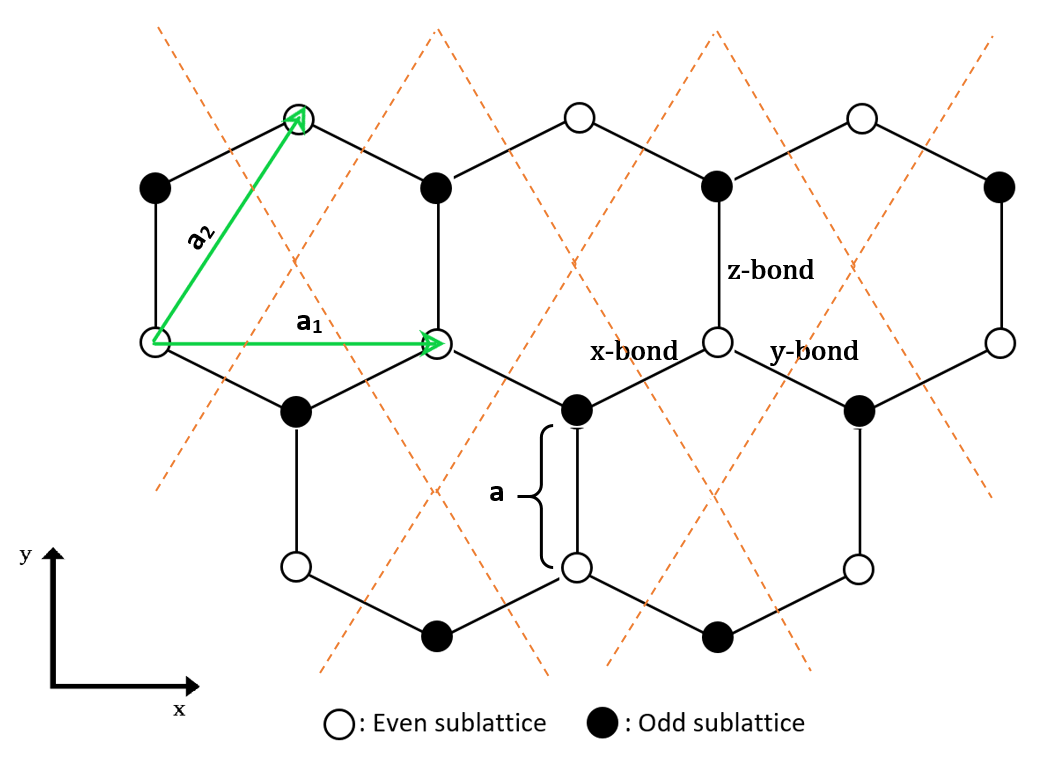
\includegraphics[width=0.7\textwidth]{./images/Final_A_2}}\\
    \subfloat[]{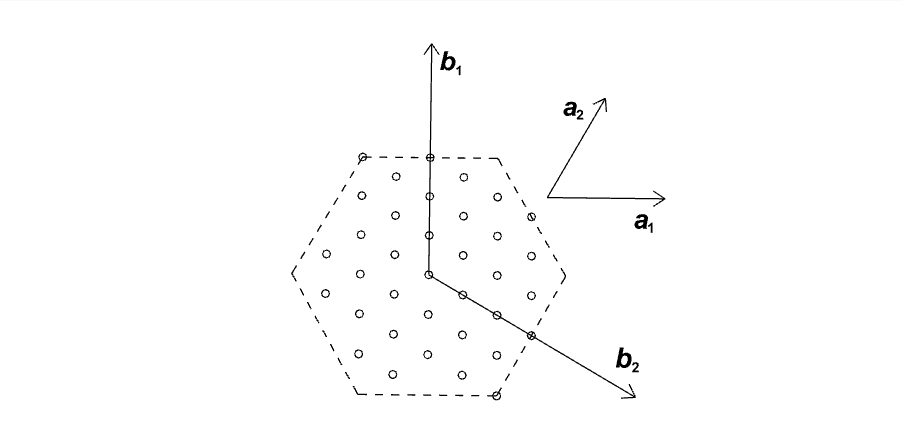
\includegraphics[width=0.8\textwidth]{./images/br_zone_v2}}
    \caption{(a) The honeycomb lattice in position space and its primitive vectors and primitive cell. (b) First Brillouin zone and primitive vectors of reciprocal lattice.}
    \label{fig:fig0}
\end{figure}

\begin{figure}[h!]
	\centering
	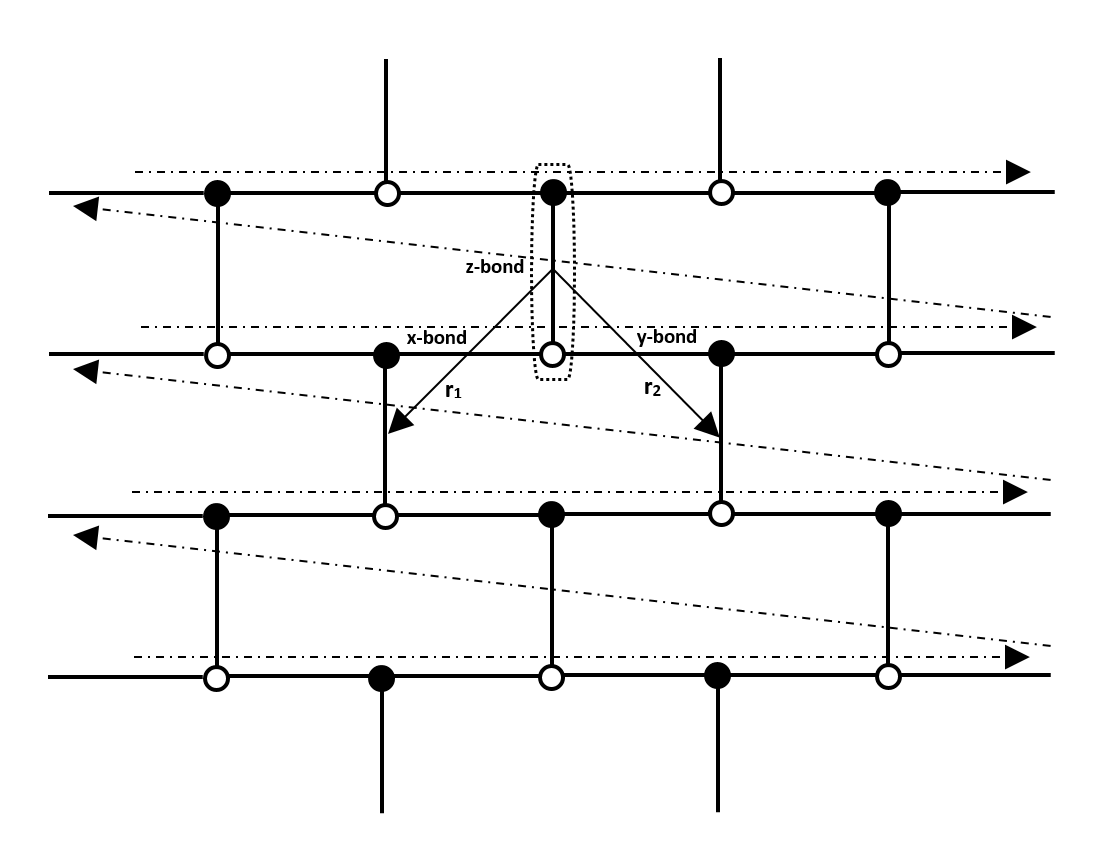
\includegraphics[width=0.8\textwidth]{./images/Jor-Wig}
	\caption{\label{jor} Brick-wall lattice and the Jordan-Wigner transformation path depicted with the dashed arrows. The $\textbf{r}_1$ and $\textbf{r}_2$ are the primitive vectors for this lattice.} 
	\label{fig:fig01}
\end{figure}

\begin{figure}[h!]
	\centering
	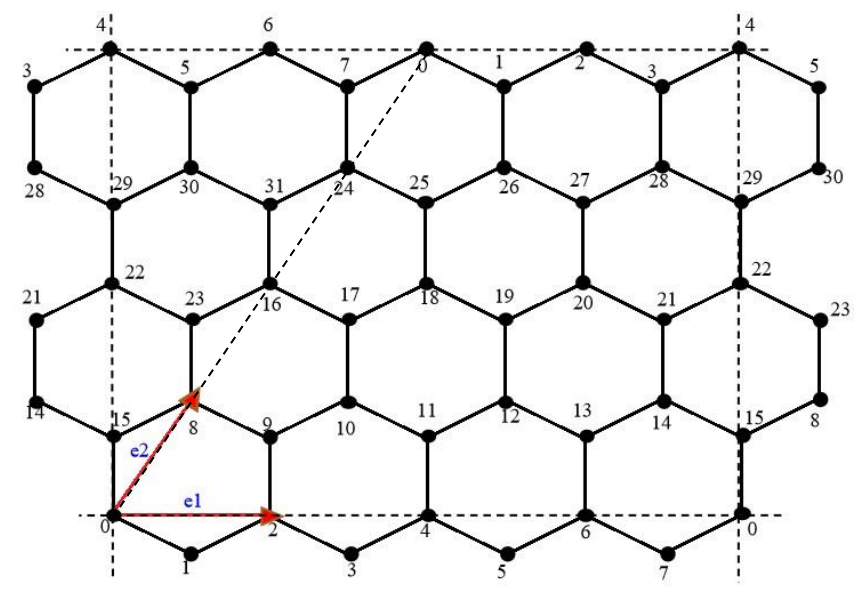
\includegraphics[width=0.8\textwidth]{./images/diag_1.png}
	\caption{\label{tab:r_space} Kitaev Honeycomb lattice model on a torus: The generators of the lattice in position space are named
	$\textbf{e}_{1}$ and  $\textbf{e}_{2}$, as shown in the image above. Hence, the lattice points are $\textbf{L} = n_{1}\textbf{e}_{1} + 
	n_{2}\textbf{e}_{2}$ with $n_{1}, n_{2} \in \mathbb{Z}$ and the above lattice is drawn for $N_{1} = N_{2} = 4 $ with toric boundary conditions.} 
	\label{fig:fig1}
\end{figure}

In this paper we apply the approach developed in \cite{Deng_2017} to the Honeycomb model. In sec.\hspace{0.2mm}\ref{sec2}, we briefly review the analytical solution of the model. In sec.\hspace{0.2mm}\ref{sec3} the mapping of the spin model to an RBM architecture is explained. In particular, we demonstrate how to calculate the groundstate and excited states of the Honeycomb model using machine learning techniques. To this end we employ the \texttt{NetKet} environment \cite{netket:2019} to train a restricted Boltzmann machine (RBM) in order to find a groundstate via gradient decent. In sec.\hspace{0.2mm}\ref{sec4} realization of vortices is discussed from both analytical and RBM language points of view. In brief, a vortex pair can be created by adjusting the parameters of the RBM and subsequent braiding can be achieved by further adjustments of parameters. Sec.\hspace{0.2mm}\ref{sec5} is dedicated to results and relevant discussions and finally we conclude in sec.\hspace{0.2mm}\ref{sec6}. An important application of the techniques developed in thi is the reconstruction of a given quantum state from simple measurements known as quantum state tomography \cite{Torlai_2018}.


% \section{The model}

% \noindent $\bullet$\hspace{4mm} The model can be mapped to a model of p-wave BCS theory with site-dependent chemical potential for spinless fermions on a square lattice \cite{2}.

% Insert the lattice pictures in here.


\section{Solution of the Model}\label{sec2}

In this section an exact solution of the system is provided and an explicit form of the groundstate energy is achieved. First of all, we Fermionize the Hamiltonian by performing a one dimensional Jordan-Wigner transformation \cite{Jordan:1928wi} defined in Equ.\hspace{0.2mm}\ref{eq:2}. A deformation of the hexagonal lattice to a brick-wall lattice (see Fig.\hspace{0.2mm}\ref{fig:fig01})  clarifies the mechanism of the Jordan-Wigner transformation and why it is one dimensional \cite{Chen_2008}. In the brick-wall lattice, each lattice site $r$ is denoted by the coordinates $(i,j)$.

\begin{equation}\label{eq:2}
	\begin{aligned}
		\sigma^{+}_{i,j} &= 2[\prod_{j'<j}\prod_{i'}\sigma^{z}_{i',j'}][\prod_{i'<i}\sigma^z_{i',j}] a^{\dagger}_{i,j}\\
		\sigma^{-}_{i,j} &= 2[\prod_{j'<j}\prod_{i'}\sigma^{z}_{i',j'}][\prod_{i'<i}\sigma^z_{i',j}] a_{i,j}\\
		\sigma^{z}_{i,j} &= 2a^{\dagger}_{i,j}a_{i,j} - 1
	\end{aligned}
\end{equation}\\

\noindent This transformation maps the Hilbert space of spins to the Hilbert space of spinless complex fermions. Using the fact that $ \sigma^{\pm} = \sigma^{x}\pm i\sigma^{y} $ one can expand the Hamiltonian in Equ.\hspace{0.2mm}\ref{eq:1} into three terms and re-write them as below \cite{Schmoll_2017}.


\begin{equation}\label{eq:3}
	\begin{aligned}
		\sigma^{x}_{i,j}\sigma^{x}_{i+1,j} &= \prod_{i'<i}\sigma^z_{i',j} (a^{\dagger}_{i,j} + a_{i,j}) \prod_{i'<i+1}\sigma^z_{i',j} (a^{\dagger}_{i+1,j} + a_{i+1,j})\\
		&= (a^{\dagger}_{i,j} + a_{i,j}) \sigma^z_{i,j} (a^{\dagger}_{i+1,j} + a_{i+1,j})\\
		&= -(a^{\dagger}_{i,j} - a_{i,j}) (a^{\dagger}_{i+1,j} + a_{i+1,j})\\
		\sigma^{y}_{i,j}\sigma^{y}_{i+1,j} &= -\prod_{i'<i-1}\sigma^z_{i',j} (a^{\dagger}_{i-1,j} - a_{i-1,j}) \prod_{i'<i}\sigma^z_{i',j} (a^{\dagger}_{i,j} - a_{i,j})\\
		&= -(a^{\dagger}_{i-1,j} - a_{i-1,j}) \sigma^z_{i-1,j} (a^{\dagger}_{i,j} - a_{i,j})\\
		&= (a^{\dagger}_{i-1,j} + a_{i-1,j}) (a^{\dagger}_{i,j} - a_{i,j})\\
		\sigma^{z}_{i,j}\sigma^{z}_{i,j+1} &=  (2a^{\dagger}_{i,j}a_{i,j} - 1) (2a^{\dagger}_{i,j+1}a_{i,j+1} - 1)\\
	\end{aligned}
\end{equation}\\

\noindent Therefore, the Hamiltonian transforms to the one in Equ.\hspace{0.2mm}\ref{eq:4}. 

\begin{equation}\label{eq:4}
	\begin{aligned}
		H= &+J_x \sum_{x-links} (a^{\dagger}_{i,j} - a_{i,j}) (a^{\dagger}_{i+1,j} + a_{i+1,j})\\
		&-J_y \sum_{y-links} (a^{\dagger}_{i-1,j} + a_{i-1,j}) (a^{\dagger}_{i,j} - a_{i,j})\\
		&-J_z \sum_{z-links} (2a^{\dagger}_{i,j}a_{i,j} - 1) (2a^{\dagger}_{i,j+1}a_{i,j+1} - 1)\\
	\end{aligned}
\end{equation}\\

\noindent The $J_x$ and $J_y$ terms are quadratic interactions in spinless fermions and are easy to solve, however, the $J_z$ term is a product of number density operators and can be further simplified by introducing the Majorana operators in Equ.\hspace{0.2mm}\ref{eq:5} \cite{Schmoll_2017}. As we will see, this simplification can be done due to the presence of the conserved quantity called plaquette operator $B_p$ \cite{Schmoll_2017}. 

\begin{equation}\label{eq:5}
	\begin{aligned}
		c_{i,j} &= i(a^{\dagger}_{i,j} - a_{i,j}) \hspace{2mm},\hspace{2mm} d_{i,j} = a^{\dagger}_{i,j} + a_{i,j} \hspace{2mm},\hspace{2mm} for \hspace{2mm} i+j=even \equiv \circ\\
		c_{i,j} &= a^{\dagger}_{i,j} + a_{i,j} \hspace{2mm},\hspace{2mm} d_{i,j} = i(a^{\dagger}_{i,j} - a_{i,j}) \hspace{2mm},\hspace{2mm} for \hspace{2mm} i+j=odd \equiv \color{black}\bullet\\
	\end{aligned}
\end{equation}\\

\noindent These operators have the following commutation relations:

\begin{equation}\label{eq:6}
	\begin{aligned}
		&c^2_{i,j} = d^2_{i,j} = 1\\
		&\{ c_{i,j},c_{i',j'} \} = \{ d_{i,j},d_{i',j'} \} = 2\delta_{ii'} \delta_{jj'}\\
		&\{ c_{i,j},d_{i',j'} \} = 0\\
	\end{aligned}
\end{equation}\\

\noindent Then, the $J_z$ term can be rewritten using the Majorana operators: 

\begin{equation}\label{eq:7}
	\begin{aligned}
		\sigma^{z}_{i,j}\sigma^{z}_{i,j+1} &=  (2a^{\dagger}_{i,j}a_{i,j} - 1) (2a^{\dagger}_{i,j+1}a_{i,j+1} - 1)\\
		&= i(id_{i,j+1}d_{i,j})c_{i,j+1}c_{i,j} 
	\end{aligned}
\end{equation}\\

\noindent Finally, using the circle indices for the odd and even lattice sites as defined in Equ.\hspace{0.2mm}\ref{eq:5} the Hamiltonian transforms to the expression in Equ.\hspace{0.2mm}\ref{eq:8}.

\begin{equation}\label{eq:8}
	\begin{aligned}
		H= &-iJ_x \sum_{x-links} c_{\circ}c_{\color{black}\bullet}\\
		&+iJ_y \sum_{y-links} c_{\color{black}\bullet}c_{\circ}\\
		&-iJ_z \sum_{z-links} (id_{\color{black}\bullet}d_{\circ})c_{\color{black}\bullet}c_{\circ}\\ 
	\end{aligned}
\end{equation}\\

\noindent If we write the Hamiltonian as a sum over unit cells we have:

\begin{equation}\label{eq:9}
	\begin{aligned}
		H= i\sum_{\textbf{r}}[J_x c_{\color{black}\bullet,\textbf{r}}c_{\circ,\textbf{r}+\textbf{r}_1} + J_y c_{\color{black}\bullet,\textbf{r}}c_{\circ,\textbf{r}+\textbf{r}_2} - J_z (id_{\color{black}\bullet,\textbf{r}}d_{\circ,\textbf{r}})c_{\color{black}\bullet,\textbf{r}}c_{\circ,\textbf{r}}]\\ 
	\end{aligned}
\end{equation}\\

\noindent where \textbf{r} is the position vector of z-bonds or unit cells  (see Fig.\hspace{0.2mm}\ref{fig:fig01}). It makes no difference in physics if we set \textbf{r} on every point along the z-bond, whether it is on even site or odd site or some where in the middle of them, that's a matter of translation! 
What will be important in what follows, is that now since we have grouped a pair of even and odd sites as an unit cell, to evaluate the summation over the unit cells, it is sufficient to just run over the even or odd sites.\\
Furthermore, the $\alpha_\textbf{r} = (id_{\color{black}\bullet,\textbf{r}}d_{\circ,\textbf{r}})$ operators are defined on each z-bond of the lattice (labled by \textbf{r}) and they commute with the Hamiltonian and are good quantum numbers.
Moreover, it can easily be shown that each plaquette operator can be written as:

\begin{equation}\label{eq:10}
	\begin{aligned}
		B_p = \sigma^y_1\sigma^z_2\sigma^x_3\sigma^y_4\sigma^z_5\sigma^x_6 = \alpha_{61}\alpha_{43}\\
	\end{aligned}
\end{equation}

\noindent On the other hand, from the Lieb's theorem \cite{Lieb_1994} we know that the groundstate manifold is obtained by setting $B_p = 1, \forall p$. 
Thus the uniform choice of $\alpha_\textbf{r}=1, \forall \textbf{r}$ corresponds to a vortex-free sector, nevertheless all configurations leading to the same sector are equivalent.\\

\noindent We also introduce a Dirac fermion on each z-link using the Majorana operators:

\begin{equation}\label{eq:11}
	\begin{aligned}
		d_\textbf{r} &= \frac{1}{2} (c_{\color{black}\bullet,\textbf{r}} - ic_{\circ,\textbf{r}})\\
		d^\dagger_\textbf{r} &= \frac{1}{2} (c_{\color{black}\bullet,\textbf{r}} + ic_{\circ,\textbf{r}})
	\end{aligned}
\end{equation}\\

\noindent Using the inverse transformation we can rewrite the Hamiltonian:

\begin{equation}\label{eq:12}
	\begin{aligned}
		H= &\sum_{\textbf{r}}[J_x (d^\dagger_{\textbf{r}} + d_{\textbf{r}})(d^\dagger_{\textbf{r}+\textbf{r}_1} - d_{\textbf{r}+\textbf{r}_1}) \\
		&+J_y (d^\dagger_{\textbf{r}} + d_{\textbf{r}})(d^\dagger_{\textbf{r}+\textbf{r}_2} - d_{\textbf{r}+\textbf{r}_2}) \\
		&+J_z \alpha_\textbf{r}(2d^\dagger_{\textbf{r}}d_{\textbf{r}}-1)]\\ 
	\end{aligned}
\end{equation}\\

\noindent The Hamiltonian is translational invariant and can be transformed to momentum space in order to be diagonalized. We define the Fourier transf for the Dirac fermion through:

\begin{equation}\label{eq:13}
	\begin{aligned}
		d_{\textbf{r}} &= \frac{1}{\sqrt{N}}\sum_\textbf{k} e^{+i\textbf{k}.\textbf{r}}d_{\textbf{k}} \\
		d^\dagger_{\textbf{r}} &= \frac{1}{\sqrt{N}}\sum_\textbf{k} e^{-i\textbf{k}.\textbf{r}}d^\dagger_{\textbf{k}} \\
	\end{aligned}
\end{equation}\\

\noindent Setting $\textbf{k} \rightarrow \textbf{-k}$ in $d^\dagger_\textbf{r}$ simplifies the calculations. We then have:

\begin{equation}\label{eq:14}
	\begin{aligned}
		\textbf{X}: \hspace{2mm} &J_x\frac{1}{N}\sum_\textbf{r}\sum_{\textbf{k},\textbf{k}'}e^{+i\textbf{k}.\textbf{r}}e^{+i\textbf{k}'.(\textbf{r}+\textbf{r}_1)}(d^\dagger_{-\textbf{k}} + d_{\textbf{k}})(d^\dagger_{-\textbf{k}'} - d_{\textbf{k}'})\\
		&= J_x\sum_{\textbf{k}} [-2cos(k_1)d^\dagger_{\textbf{k}}d_{\textbf{k}} + isin(k_1)(d^\dagger_{\textbf{k}}d^\dagger_{-\textbf{k}}-h.c.)]\\
		\textbf{Y}: \hspace{2mm} &J_y\frac{1}{N}\sum_\textbf{r}\sum_{\textbf{k},\textbf{k}'}e^{+i\textbf{k}.\textbf{r}}e^{+i\textbf{k}'.(\textbf{r}+\textbf{r}_2)}(d^\dagger_{-\textbf{k}} + d_{\textbf{k}})(d^\dagger_{-\textbf{k}'} - d_{\textbf{k}'})\\
		&= J_y\sum_{\textbf{k}} [-2cos(k_2)d^\dagger_{\textbf{k}}d_{\textbf{k}} + isin(k_2)(d^\dagger_{\textbf{k}}d^\dagger_{-\textbf{k}}-h.c.)]\\
		\textbf{Z}: \hspace{2mm} &J_z\frac{1}{N}\sum_\textbf{r}\sum_{\textbf{k},\textbf{k}'}e^{+i\textbf{k}.\textbf{r}}e^{+i\textbf{k}'.\textbf{r}}(2d^\dagger_{-\textbf{k}}d^\dagger_{\textbf{k}'}-1)\\
		&= J_z\sum_{\textbf{k}} 2d^\dagger_{\textbf{k}}d_{\textbf{k}}-J_zN.\\
	\end{aligned}
\end{equation}\\

\noindent For the above equation we used the orthogonality relation in Fourier transformation:

\begin{equation}\label{eq:15}
	\begin{aligned}
		\sum_\textbf{r} e^{i(\textbf{k}+\textbf{k}').\textbf{r}} = N\delta(\textbf{k} + \textbf{k}')
	\end{aligned}
\end{equation}\\

Using all previous transformations we obtain a Hamiltonian which is quadratic in the Dirac fermions living on each of the unit cells along the z-links:

\begin{equation}\label{eq:16}
	\begin{aligned}
		H = \sum_\textbf{k}[\epsilon_\textbf{k}d^\dagger_{\textbf{k}}&d_{\textbf{k}} + \frac{1}{2}(i\Delta_\textbf{k}d^\dagger_{\textbf{k}}d^\dagger_{-\textbf{k}}-i\Delta_\textbf{k}d_{-\textbf{k}}d_{\textbf{k}})]-J_zN\\
		\epsilon_\textbf{k} &= 2[J_z-J_xcos(k_1)-J_ycos(k_2)]\\
		&\Delta_\textbf{k} = 2[J_xsin(k_1)+J_ysin(k_2)]\\
	\end{aligned}
\end{equation}\\

\noindent By applying a unitary Bogoliubov transformation, we diagonalize the Hamiltonian which can be written as:

\begin{equation}\label{eq:17}
	\begin{aligned}
		H &= \sum_\textbf{k} \frac{1}{2} 
		\begin{pmatrix}
			\gamma^\dagger_\textbf{k} & \gamma_{\textbf{-k}}
		\end{pmatrix}
		\begin{pmatrix}
			E_\textbf{k} & 0\\
			0 & -E_\textbf{k}
		\end{pmatrix}
		\begin{pmatrix} \gamma_\textbf{k} \\ \gamma^\dagger_{\textbf{-k}} \end{pmatrix}\\
		&= \sum_\textbf{k}E_\textbf{k}(\gamma^\dagger_\textbf{k}\gamma_{\textbf{k}}-\frac{1}{2}).
	\end{aligned}
\end{equation}\\

\noindent with a groundstate energy of $E_{GS} = -\frac{E_\textbf{k}}{2}$.

\section{Restricted Boltzmann Machine Representation}\label{sec3}

With the ever growing applications of neural networks in sciences and the emergent new technologies to deploy and build physical neural networks, this is the right time to investigate potential applications of them in condensed matter systems. Recently, a new approach has been proposed for simulating topological quantum states using neural networks \cite{Deng_2017}. In this section we use the same approach to map the Honeycomb Kitaev model to a restricted Boltzmann machine (RBM). There are many reasons why an RBM is chosen. This particular architecture has proved to be effective in many tasks such as dimensional reduction, classification, regression, collaborative filtering, feature learning and topic modeling and moreover a general theorem shows that RBMs are universal approximators of discrete distributions \cite{LeRouxBengio}.

Having a set of spins on a lattice, $\Xi=(\sigma_{1},\sigma_{2},\cdots\sigma_{N})$ (in our case the Jordan-Wigner chain of spins), our goal is to use an RBM to reduce the dimensionality of the Hilbert space and estimate the energy of the system in both groundstate and excited states and classify different topological phases of the model. An RBM is a short range feed-forward neural network with two layers. The first layer (visible layer) has $N$ nodes which are representing the physical spins in the Hamiltonian and the second layer (hidden layer) has $M$ binary valued nodes (architecture of the network is shown in Fig.\ref{rbm-arc}). 

\begin{figure}[!htb]
	\centering
	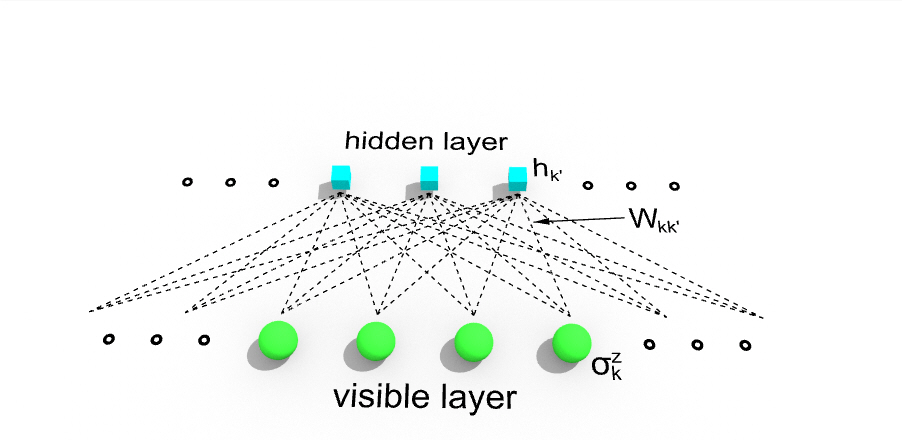
\includegraphics[width=0.8\textwidth]{./images/rbm}
	\caption{\label{rbm-arc} Fully connected Restricted Boltzmann machine architecture.}
\end{figure}

The quantum state of the Honeycomb model, up to an irrelevant normalization factor, can be written as 

\begin{equation}\label{eq:19_0}
    |\Phi\rangle=\sum_{\Xi}\Phi_{M}(\Xi;\Omega)|\Xi\rangle
\end{equation}{}

where

\begin{equation}\label{eq:19_1}
    \begin{aligned}
        \Phi_{M}(\Xi;\Omega) &=  \sum_{\{h_{k}\}}e^{\sum_{k}a_{k}\sigma_{k}^{z}+\sum_{k'}b_{k'}h_{k'}+\sum_{kk'}W_{kk'}h_{k}\sigma_{k'}^{z}}\\
        &= e^{\sum_k a_k \sigma_k^z} \times \prod_{k'} \cosh \left(\sum_k W_{kk'} \sigma_k^z + b_{k'} \right)
    \end{aligned}
\end{equation}\\

To obtain the second equality we used the values for $\{h_{k}\}=\{-1,1\}^{M}$ which is the set of possible configurations of hidden layer nodes and the $\Omega=(a_{k},b_{k'},W_{kk'})$ is the set of weights and biases of the RBM which should be trained in such a way that the final RBM state represents the desired quantum state of the model (i.e. groundstate or the excited states). The combined number of weight and bias parameters and nodes is polynomial in system size and computationally feasible.

% If the visible and hidden layers of the network are fully connected, training the network for large lattice sizes is not computationally feasible. Therefore, we just use locally connected RBM in which the number of weight parameters and nodes in layers is linear in system size. 

Mapping of the model to RBM was done using the machinery already developed in the \texttt{NetKet} software package \cite{netket:2019}. In order to train the network, the parameter space of the network was sampled using the Metropolis algorithm and the optimization iterations are based on stochastic gradient descent algorithm. 

\section{Braiding}\label{sec4}

In this section we want to explore the possibility to create anionic excitations in the RBM representation and describe anyon braiding. Such a representation is important for various reasons, in particular for performing quantum computation \cite{Nayak_2008}. 

First of all, let us describe the creation of these quasi-particles by starting with a groundstate sector and then subsequently changing the eigenvalue of the $B_p$ operators from +1 to -1 locally and in the region that we want to realize the vortices in the system. 
In an arbitrary configuration of spins (not necessarily in the groundstate sector) it is easy to prove that $\prod B_p = +1 ,\forall p$. Hence, we can just build the vortices in pairs. For example, if you apply the operator $\hat{O}_1$ to the groundstate,  it produces two vortices in plaquettes 1 and 2 (see Fig.\hspace{0.2mm}\ref{fig:anyons}). \todo{Do we need a reference here or are these ideas completely new?}

\begin{equation}\label{eq:18}
    \hat{O}_1 = \exp{(-i\frac{\pi}{2}\hat{\sigma}^{z}_a)}
\end{equation}{}

Another possibility is to apply the following operator 

\begin{equation}\label{eq:19}
    \hat{O}_2 = \exp{(-i\frac{\pi}{2}\hat{\sigma}^{x}_a)}\exp{(-i\frac{\pi}{2}\hat{\sigma}^{y}_b)}~,
\end{equation}{}

which produces two vortices along the $\hat{z}$ direction in plaquettes 3 and 4.

\begin{figure}[!htb]
    \centering
    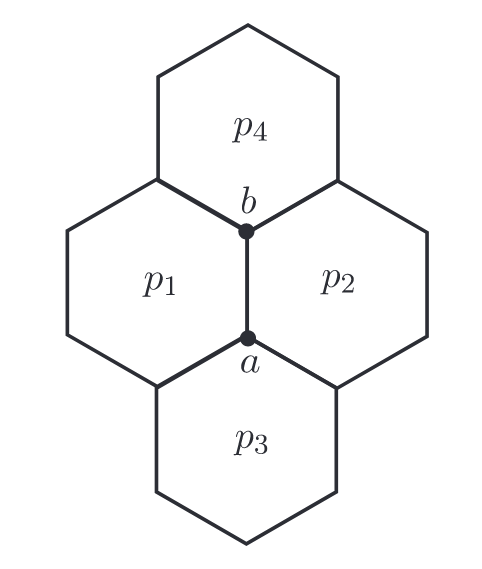
\includegraphics[width=0.3\textwidth]{./images/anyons.png}
    \caption{Caption}
    \label{fig:anyons}
\end{figure}{}

The reason why these operators can produce vortices in the system can be explained by re-writing the Hamiltonian of the system in terms of Majorana fermions. Kitaev originally solved the Hamiltonian through this approach. The disadvantage of this approach in comparison to what was done above is that when the Hamiltonian is mapped to Majorana fermions, there are unphysical states in the system which need to be projected out. This will be clear as we go along.\\

We assume that there are two fermionic modes living on each lattice site corresponding to the four creation and annihilation operators $a^\dagger_{m,i}$ and $a_{m,i}$, where $m\in \{1,2\}$ is the index for the modes and $i$ is the index for the lattice sites. Here unlike before, we use one index for lattice site to avoid unnecessary complications. Then we will separate the imaginary and real parts of these operators, to define the Majorana fermions as below

\begin{equation}\label{eq:20}
    \begin{aligned}
        & c_i = a_{1,i} + a^\dagger_{1,i} \\
        & b^x_i = i(a^\dagger_{1,i} - a_{1,i}) \\
        & b^y_i = a_{2,i} + a^\dagger_{2,i} \\
        & b^z_i = i(a^\dagger_{2,i} - a_{2,i})
    \end{aligned}
\end{equation}{}\\

Notice that the spins have a two dimensional space (being up or down) and now that we are representing them with four Majorana modes (two complex fermionic modes), we need to project out the unphysical states. The Fock space of the complex fermionic modes can be represented as $\{\ket{00}, \ket{01}, \ket{10}, \ket{11}\}$. We make the following correspondence between the states of spins and fermions 

\begin{equation}\label{eq:21}
    \begin{aligned}
        & \ket{\uparrow} = \ket{00} \\
        & \ket{\downarrow} = \ket{11}
    \end{aligned}
\end{equation}{}\\

We can define the projector $P_i$ on site $i$ to do this job for us

\begin{equation}\label{eq:22}
    \begin{aligned}
        P_i = \frac{1+D_i}{2} \hspace{2mm}\text{where}\hspace{2mm} D_i = (1-2a^\dagger_{1,i}a_{1,i})(1-2a^\dagger_{2,i}a_{2,i}) = b^x_i b^y_i b^z_i c_i~.
    \end{aligned}
\end{equation}{}\\

One can easily show that the relation between Majorana operators and the original Pauli operators is as follows

\begin{equation}\label{eq:23}
    \begin{aligned}
        \sigma^\alpha_i = i b^\alpha_i c_i \hspace{3mm}\text{for}\hspace{3mm} \alpha\in \{x,y,z\}~.\\
    \end{aligned}
\end{equation}{}\\

In fact, by the above projection, we satisfied the extra condition coming from the algebra of Pauli matrices, $-i\sigma^x_i\sigma^y_i\sigma^z_i = b^x_i b^y_i b^z_i c_i = \mathbb{1}$. Therefore, the eigenvalue of the projector $P_i$ for physical states is 1 and for unphysical states is 0.

Using Equ.\hspace{0.2mm}\ref{eq:23} the Hamiltonian can be written in terms of Majorana operators as

\begin{equation}\label{eq:24}
	\begin{aligned}
		H = \frac{i}{2} \sum_{i,j} A_{ij} c_i c_j \hspace{2mm}\text{where}\hspace{2mm} A_{ij} = J_{ij} u_{ij} \hspace{2mm}\text{and}\hspace{2mm} u_{ij} = i b^\alpha_i b^\alpha_j \hspace{2mm}\text{with}\hspace{2mm} \alpha\in \{x,y,z\}~.
	\end{aligned}
\end{equation}\\

The $u_{ij}$ are antisymmetric Hermitian link operators with eigenvalues $\pm 1$

\begin{equation}\label{eq:25}
	\begin{aligned}
		u_{ij} = -u_{ji}, \hspace{2mm} u^2_{ij} = 1, \hspace{2mm}, u^\dagger_{ij} = u_{ij}
	\end{aligned}
\end{equation}\\

The link operators commute with the Hamiltonian, $[H, u_{ij}] = 0$, so they are local symmetries. In this form, the Hamiltonian is representing a tight binding model of free Majorana fermions hopping along the lattice, with tunneling couplings that depend on the eigevalues of link operators which can be thought of as a classical $\mathbb{Z}_2$ gauge field. One can assign a configuration $\{u\}$ to all link operators and diagonalize the resulting quadratic Hamiltonian in Majorana operators directly and obtain the spectrum and groundstate energy for $H\{u\}$. But which configuration $\{u\}$ corresponds to the global minimum of the energy? This question has been answered by Lieb (1994) \cite{kour2014real}. The groundstate lies in the sector with $B_p = 1 \hspace{2mm} \forall ~p$ and since the $B_p$ operators are the only gauge invariant objects, every gauge fixing choice $\{u\}$ which leads to this particular configuration for $B_p$ is equivalent. Therefore, our goal is to find a configuration $\{u\}$ which leads to $B_p = 1 \hspace{2mm} \forall ~p$. 

Next, we define the vortex operator $W_p$ as

\begin{equation}\label{eq:26}
	\begin{aligned}
		W_p = \prod_{(i,j)\in \partial P} u_{ij} \hspace{2mm}\text{where}\hspace{2mm}
		\left\{
		\begin{array}{l}
            i  \in \hspace{2mm} \text{even sublattice} \\
            j  \in \hspace{2mm} \text{odd sublattice}
        \end{array}
        \right.~.
	\end{aligned}
\end{equation}\\

The vortex operator can be simplified as below

\begin{equation}\label{eq:27}
	\begin{aligned}
		W_p &= u^x_{12}u^y_{32}u^z_{34}u^x_{54}u^y_{56}u^z_{16} \\
		&= -(i)^6 c^x_1 c^x_2 c^y_2 c^y_3 c^z_3 c^z_4 c^x_4 c^x_5 c^y_5 c^y_6 c^z_6 c^z_1 \\
		&= \sigma^y_1 D_1 \sigma^z_2 D_2 \sigma^x_3 D_3 \sigma^y_4 D_4 \sigma^z_5 D_5 \sigma^x_6 D_6 ~,
	\end{aligned}
\end{equation}\\

where we used $i c^x_j c^y_j = -\sigma^z_j D_j$ and cyclic permutations. Considering the fact that $[W_p, H] = [W_p, D_i] = 0$, in the physical subspace where $D_j = 1$ we recover $W_p = B_p$. Therefore, the uniform choice of $u_{ij}=1$ for every link will lead us to the groundstate in the extended (not yet projected) space with $B_p = 1$. In order to find the physical groundstate, we apply the global projector $\mathbf{D}$ to project out the unphysical states

\begin{equation}\label{eq:28}
	\begin{aligned}
		\ket{\psi_w}_{physical} = \mathbf{D} \ket{\psi_u}_{extended},  \hspace{2mm}\text{where}\hspace{2mm} \mathbf{D} = \prod^N_{i=1} P_i
		\end{aligned}
\end{equation}\\

Now we are at a point to explain in detail why the operators $\hat{O}_1$ and $\hat{O}_2$ can create vortices in the system. As mentioned earlier, if we flip the sign of eigenvalue of vortex operator at p, a vortex will be created in the system. Looking back at Equ.\hspace{0.2mm}\ref{eq:26}, we see that the vortex configuration $\{W_p\}$ is created by fixing the gauge at every link $\{u_{ij}\}$. Therefore, by changing the link operators, we can move between vortex sectors. Starting from a vortex-free sector with all link operators being $+1$, applying the $\hat{O}_1$ on site $a$ will leave the $\sigma^z_a$ untouched while flipping the $\sigma^x_a$ and $\sigma^y_a$. Consequently, this will change the sign of the eigenvalue of the $u_{ij}$ for x-link and y-link attached to site $a$, leaving the system with $B_{p_1} = -1$ and $B_{p_2} = -1$. We can also move the vortices around in the system, by consecutively applying these operators on the particular sites in a path for which we want to move the vortices along. As an example, the red path shown in the Fig.\hspace{0.2mm}\ref{fig:string} corresponds to the operator

\begin{equation}\label{eq:29}
	\begin{aligned}
		\hat{O} = \exp{(-i\frac{\pi}{2}\sigma^z_i)} \exp{(-i\frac{\pi}{2}\sigma^x_j)}
		\end{aligned}
\end{equation}

\begin{figure}[!htb]
    \centering
    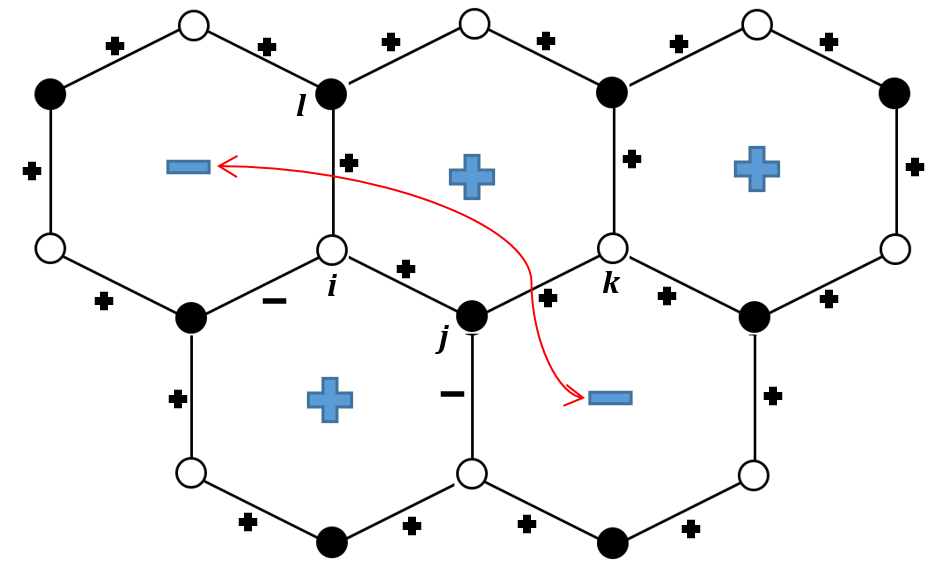
\includegraphics[width=0.7\textwidth]{./images/Anyons_Strings}
    \caption{Two vortices connected by a string operator passing through several links. The white dots denote even lattice sites while the black dots are odd ones. By convention, the string operator is built up from operators acting on even sites.}
    \label{fig:string}
\end{figure}{}

In general, we can define string operators to move the vortices anywhere in the system along the string, similar to the example above. To create such a string operator is straightforward now. If the string passes through a link, we need to apply an operator on one of the sites connected to that $\alpha-link$ which carries $\sigma^\alpha$ in the exponent. Before continuing, we need to make a convention. A sharp reader might point out that applying the operator $\hat{O}^{'} = \exp{(-i\frac{\pi}{2}\sigma^z_l)} \exp{(-i\frac{\pi}{2}\sigma^x_k)}$ instead of $\hat{O}$ creates the same pair of vortices in the system. For consistency reasons, we therefore use the convention that if a string is passing through a link, the corresponding string operator is built up by picking the even site on the link. Having said all of this,  a generic string operator is defined as

\begin{equation}\label{eq:29}
	\begin{aligned}
		\hat{S} = \prod_{\alpha-links} \exp{(-i\frac{\pi}{2}\hat{\sigma}^\alpha_\circ)}~.
		\end{aligned}
\end{equation}

This string operator will create two vortices at the ending points of the string which passes through the $\alpha-links$. The manipulation of link operators using these string operators is practically equivalent to changing the sign of the couplings $J_{ij}$ corresponding to the link $u_{ij}$ in the definition of the $A_{ij}$ (see Equ.\hspace{0.2mm}\ref{eq:24}). Therefore, in the RBM language one can simply redefine the Hamiltonian with the desired signs of $J_{ij}$ for a particular vortex sector and then try to find the RBM representation for this new Hamiltonian through the approach explained in section 3. The only practical disadvantage of this vortex realization approach is that it is computationally expensive as the RBM should be trained again from scratch to find the representation for the excited state. An ideal approach is that, given the representation for groundstate, we would be able to directly and without further optimization steps find the representation for the excited state. 

In principle, it is possible to directly manipulate the weight and bias parameters of the RBM,  $\Omega=(a_{k},b_{k'},W_{kk'})$ to realize the vortices and find the excited state representation. Looking at Equ.\hspace{0.2mm}\ref{eq:19_1}, we notice that there is a symmetry between the eigenvalues of physical spins and the value of parameters of the RBM. In other words, flipping a particular spin in site $k$ is equivalent to flipping the sign of the RBM parameter sitting next to the $\sigma^{\alpha}_k$ in Equ.\hspace{0.2mm}\ref{eq:19_1} and/or adding a phase to it. In general, for a string operator $\hat{S}_a = \exp{(-i\frac{\pi}{2}\hat{\sigma}^{\alpha}_a)}$ we have:

\begin{equation}\label{eq:29_1}
	\begin{aligned}
		\hat{S}~|\Phi\rangle &= (-i\hat{\sigma}^{\alpha}_a)\sum_{\Xi}\Phi_{M}(\Xi;\Omega)|\Xi\rangle\\
		&= \sum_{\Xi} e^{[(-1)^{\delta(\alpha-z)-1} a_a -i\frac{\pi}{2}\sigma^{z}_a]\sigma^{z}_a + \sum_{k\neq a} a_k \sigma_k^z} \times \\ &\prod_{k'} \cosh \left((-1)^{\delta(\alpha-z)-1} W_{ak'} \sigma_a^z + \sum_{k\neq a} W_{kk'} \sigma_k^z + b_{k'} \right) \hat{\sigma}^{\alpha}_a~|\Xi\rangle
	\end{aligned}
\end{equation}

Therefore, applying $\hat{S}_a$ on RBM state, is equivalent to multiplying the bias parameter $a_a$ and weight parameters $W_{ak'}~\forall k'$ by $(-1)^{\delta(\alpha-z)-1}$ and then manually adding a $(-i\frac{\pi}{2}\sigma^{z}_a)$ phase angle to $a_a$, where $\sigma^{z}_a \in \{-1,+1\}$ is the eigenvalue of the $z$ component of the spin on site $a$. The presence of the $(-1)^{\delta(\alpha-z)-1}$ factor is to ensure that when $\alpha=x$ or $y$, the $\hat{\sigma}_a^{z}$ eigenvalue is multiplied by a minus sign. 


\section{Results and Discussion}\label{sec5}

% \begin{figure}[h!]
% 	\centering
% 	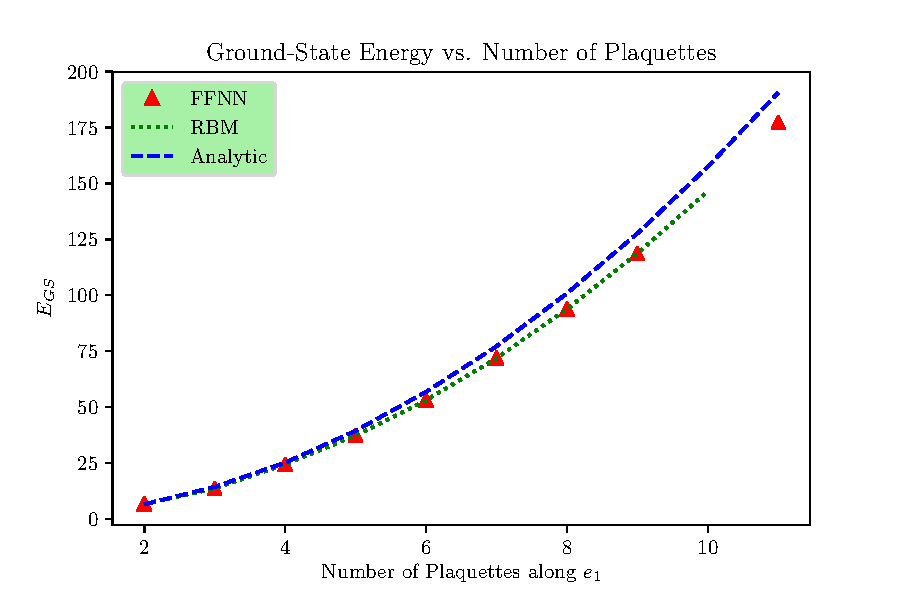
\includegraphics[width=0.8\textwidth]{E_GS.pdf}
% 	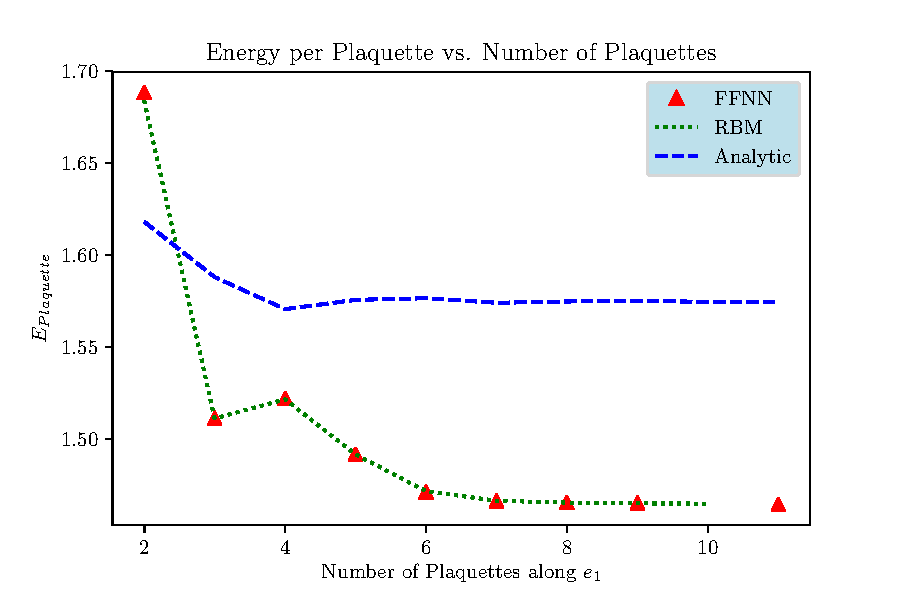
\includegraphics[width=0.8\textwidth]{E_p.pdf}
% 	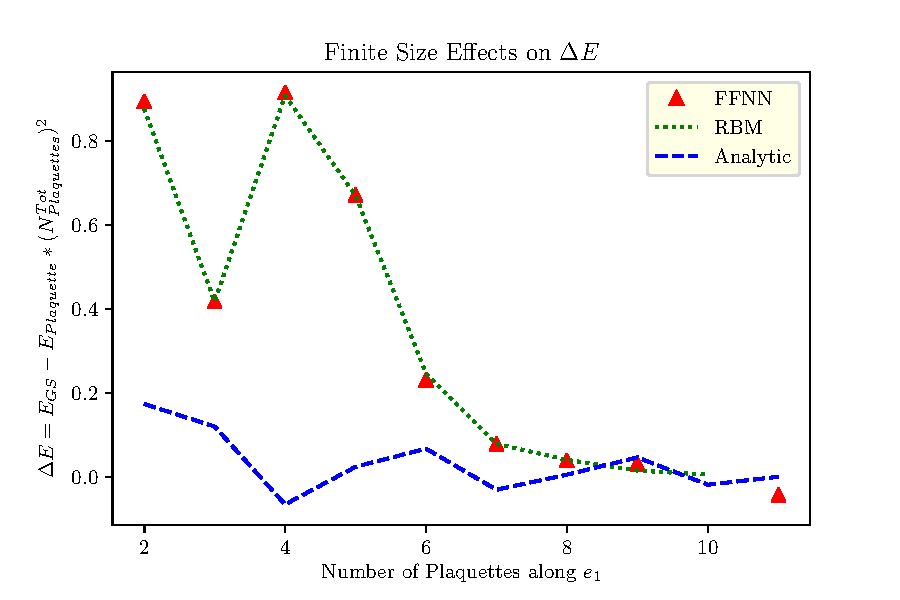
\includegraphics[width=0.8\textwidth]{DeltaE.pdf}
% 	\includegraphics[width=0.8\textwidth]{plots.pdf}
% 	\caption{\label{tab:r_space} Kitaev Honeycomb lattice model on a torus: The generators of the lattice in position space are named as
% 	$\textbf{e}_{1}$ and  $\textbf{e}_{2}$, as shown in the image above. Hence, the lattice points are $\textbf{L} = n_{1}\textbf{e}_{1} + 
% 	n_{2}\textbf{e}_{2}$ with $n_{1}, n_{2} \in \mathbb{Z}$ and the above lattice is drawn for $N_{1} = N_{2} = 4 $ with toric boundary conditions.} 
% \end{figure}

\subsection{Groundstate}

In this section, we present the results for the groundstate energy estimation of different system sizes for the proposed mapping in the section 3. These results are also compared to the exact analytical expression given in Equ.\hspace{0.2mm}\ref{eq:17}. The absolute value of the energies is plotted in Fig.\hspace{0.2mm}\ref{tab:r_space}. 

The RBM has the simple fully-connected and two-layered architecture with an optimized value of $\alpha = \frac{num_{h}}{num_{v}} = 2$ which is the ratio of number of hidden nodes to the number of visible nodes. For lower values of $\alpha$ the network does not give an accurate estimation of energies, while the larger values cause over-fitting and again inaccurate results. For training, the configuration space of the network has been sampled for hundreds of  times, depending on the lattice size, using Metropolis algorithm. Moreover, the stochastic gradient descent algorithm has been used for optimization for enough number of iterations such that the network converge to a low enough minima of the energy landscape.

\begin{figure}[!htb]
	\centering
	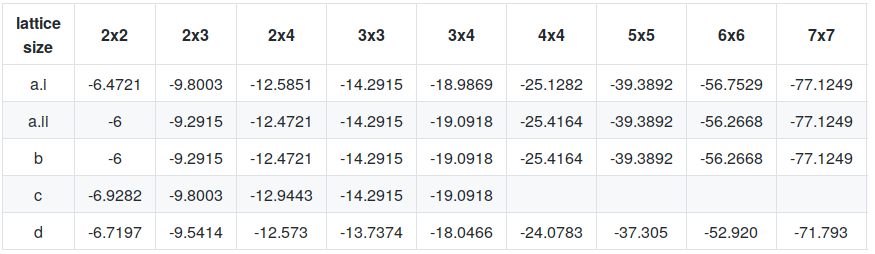
\includegraphics[width=0.5\textwidth]{./images/gs_tbl.png}
	\includegraphics[width=0.7\textwidth]{./images/plots.pdf}
	\caption{\label{tab:r_space} Numerical results for groundstate energy calculation using Restricted Boltzmann Machines (RBM) 
	and Feed-Forward Neural Networks (FFNN) compared to the analytically obtained groundstate energy using Equ.\hspace{0.2mm}\ref{eq:16}.} 
\end{figure}

Based on the results obtained for the energy of the state of system, training of the network was tested and optimized by changing the learning rate for different training phases and iteration numbers. However, the outcome was not considerably changed and improved and it seems that the above results are the most accurate results one can get for this particular architecture of network. 

In order to check the effect of relative number of hidden and visible nodes on the outcome of the network, different values for $\alpha$ were tested, keeping other parameters fixed. The $\alpha$ parameter was changed just by changing the number of hidden nodes for a fixed system size (and hence fixed visible layer size) and the results are outlined in the table below, including the number of free parameters of the network and the time needed for the network to be trained. The exact analytical energy for the selected spin system is $-39.3892$.

\begin{figure}[!htb]
	\centering
	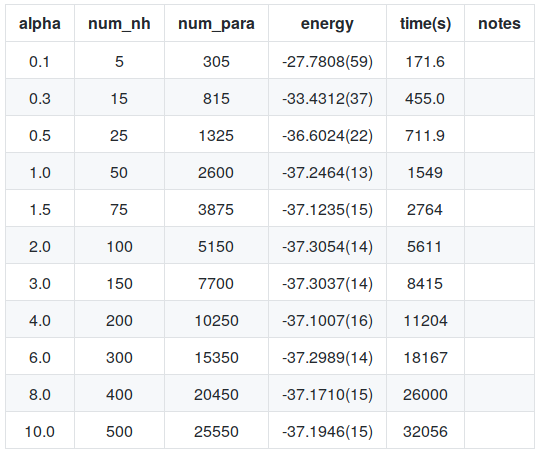
\includegraphics[width=0.6\textwidth]{./images/alpha.png}
	\caption{\label{tab:alpha} Numerical results for the number of hidden nodes and its influence on energy calculations. $\alpha = \frac{num_{h}}{num_{v}}$.} 
\end{figure}

    -- 2 is the most suitable value for alpha. If it is too low, the fitting performace is not good; too high overfit will happen. \\
    -- The training time is approximately proportional to the number of parameters. For each additional parameter, the training time is increased by about 1 second. \\
    -- The result of RBM is still far away from the analytic result. \\

\textbf{The performance of FFNN}

Below is the result of FFNN with one layer. As the structure of ffnn is similar to that of a no-visible-bias RBM(reffered as novb RBM below), the performance of one-layer FFNN is compared to that of no-visible-bias RBM.

\begin{figure}[!htb]
	\centering
	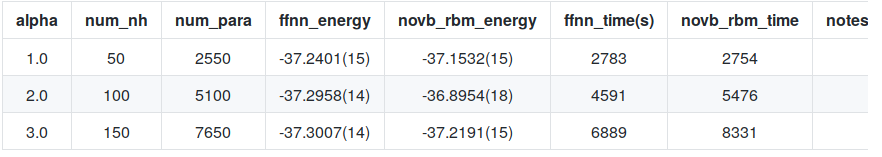
\includegraphics[width=0.8\textwidth]{./images/ffnn.png}
	\caption{\label{tab:ffnn} FFNN analysis.} 
\end{figure}    

    -- FFNN trains faster than RBM and performs better than RBM with no bias.\\
    -- But FFNN's result again far away from the analytic one. \\

Deep FFNNs with 2 and 3 layers are also tried. But some bugs seem happen, the energies stay at -25. It will be studied later.

\subsection{Excited States: Realization of Anyons}

\textbf{Create Vortex and Measure its energy}

There are three theoretically equivalent method to create vortices

    (a) modifing parameters of RBM \\
    (b) creating a auxiliary Hamiltonian and train again \\
    (c) transforming into auxiliary fermion and fixing $u_{ij}$s (Kitaev and Pachos) \\
    
I will first triple check using 3x3 lattice. The numeric result of gs energy of 3x3 lattice is -13.7166(2), the theoretical gs energy is -14.2915. The results is as the table below.

\begin{figure}[!htb]
	\centering
	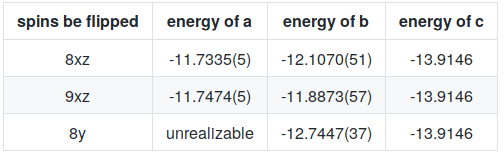
\includegraphics[width=0.8\textwidth]{./images/3x3.png}
	\caption{\label{tab:3x3} 3x3 lattice analysis.} 
\end{figure}

* There is a wired thing in method c, need to discuss!

Method a is more stable than method b. Both of method a and b is far from the correct result, method c. As the time they take, method c takes several ms to finish; method a and b take several minutes and method a is 3 or 4 times faster than method b.

Now turn to larger lattice size, say, 7x7. It is wired in computation of method a that all these computations take exactly 1.5 days. By exactly, I means the error is at most 4 mins. The results are as below.

\begin{figure}[!htb]
	\centering
	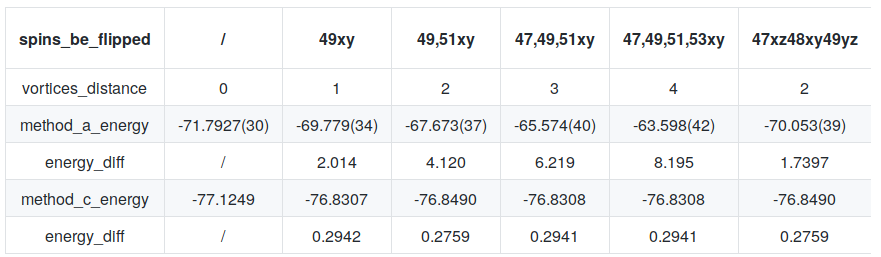
\includegraphics[width=0.8\textwidth]{./images/vort_dis.png}
	\caption{\label{tab:vort_dis} Vortex vs. Distance analysis.} 
\end{figure}

It is worth to evaluate energy of vertices by method c for more large systems.

\begin{figure}[!htb]
	\centering
	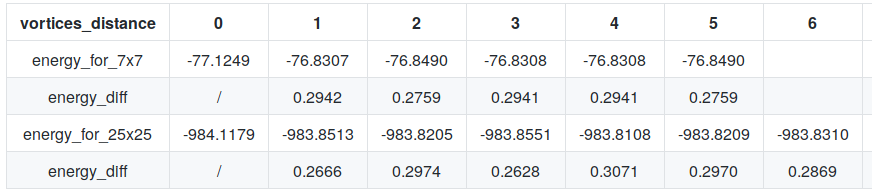
\includegraphics[width=0.8\textwidth]{./images/vort_dis_c.png}
	\caption{\label{tab:vort_dis} Vortex vs. Distance analysis: Method C.} 
\end{figure}

% \section{Topological Quantum Phase Transition}

%\subsection{Implementation in \textit{Intel-QS}}


\section{Conclusion}\label{sec6}
\label{sec:conclusion}


\section{Acknowledgement}
YMSC, Martin Duy Tat, 

%\subsection{Figures}
%\lipsum[10] 
%See Figure \ref{fig:fig1}. Here is how you add footnotes. \footnote{Sample of the first footnote.}
%\lipsum[11] 

%\begin{figure}[h!]
%  \centering
%  %\includegraphics[width=2cm]{./images/arch}
%  \fbox{\rule[-.5cm]{4cm}{4cm} \rule[-.5cm]{4cm}{0cm}}
%  \caption{Sample figure caption.}
%  \label{fig:fig20}
%\end{figure}

%\subsection{Tables}

%\begin{table}[h!]
% \caption{Sample table title}
%  \centering
%  \begin{tabular}{lll}
%    \toprule
%    \multicolumn{2}{c}{Part}                   \\
%    \cmidrule(r){1-2}
%    Name     & Description     & Size ($\mu$m) \\
%    \midrule
%    Dendrite & Input terminal  & $\sim$100     \\
%    Axon     & Output terminal & $\sim$10      \\
%    Soma     & Cell body       & up to $10^6$  \\
%    \bottomrule
%  \end{tabular}
%  \label{tab:table}
%\end{table}

%\lipsum[5]
%\begin{equation}
%\xi _{ij}(t)=P(x_{t}=i,x_{t+1}=j|y,v,w;\theta)= {\frac %{\alpha _{i}(t)a^{w_t}_{ij}\beta %_{j}(t+1)b^{v_{t+1}}_{j}(y_{t+1})}{\sum _{i=1}^{N} \sum %_{j=1}^{N} \alpha _{i}(t)a^{w_t}_{ij}\beta %_{j}(t+1)b^{v_{t+1}}_{j}(y_{t+1})}}
%\end{equation}

%\subsubsection{Headings: third level}
%\lipsum[6]

%\paragraph{Paragraph}
%\lipsum[7]


%\lipsum[8] \cite{intel,qperc} and see \cite{hard}.

%The documentation for \verb+natbib+ may be found at
%\begin{center}
%  \url{http://mirrors.ctan.org/macros/latex/contrib/natbib/natnotes.pdf}
%\end{center}
%Of note is the command \verb+\citet+, which produces citations
%appropriate for use in inline text.  For example,
%\begin{verbatim}
%   \citet{hasselmo} investigated\dots
%\end{verbatim}
%produces
%\begin{quote}
%  Hasselmo, et al.\ (1995) investigated\dots
%\end{quote}

%\begin{center}
%  \url{https://www.ctan.org/pkg/booktabs}
%\end{center}



%\lipsum[12]
%See awesome Table~\ref{tab:table}.



%\subsection{Lists}
%\begin{itemize}
%\item Lorem ipsum dolor sit amet
%\item consectetur adipiscing elit. 
%\item Aliquam dignissim blandit est, in dictum tortor gravida eget. In ac rutrum magna.
%\end{itemize}


 \bibliographystyle{JHEP}     
 {\footnotesize{\bibliography{references}}}



\end{document}
% The $\{h_{k}\}=\{-1,1\}^{M}$ is the set of possible configurations of hidden layer nodes and the $\Omega=(a_{k},b_{k'},W_{kk'})$ is the set of weights of the RBM which should be trained in such a way that the final RBM state represents the desired quantum state of the model (i.e. groundstate or the excited states).

